% eqedoc.tex V2.0, 27 March 2010

\documentclass[times]{eqeauth}

\usepackage{amsmath}
\usepackage{moreverb}
\usepackage{subfigure}
\usepackage{bbm}
%\usepackage{epsfig}
\usepackage[comma,square,sort&compress,numbers]{natbib}
\renewcommand{\bibnumfmt}[1]{{#1}.}
\usepackage{epstopdf}
\epstopdfsetup{outdir=./FIGS/}
\usepackage{setspace}
\usepackage{color}
\renewcommand{\topfraction}{0.85}
\renewcommand{\textfraction}{0.1}
\renewcommand{\floatpagefraction}{0.85}
\usepackage{mathtools}
\DeclarePairedDelimiter{\diagpars}{(}{)}
\newcommand{\diag}{\operatorname{diag}\diagpars}
\newcommand{\norm}[1]{\displaystyle \left\| #1 \right\|}
\newcommand{\hilight}[1]{\colorbox{yellow}{#1}}

\usepackage[dvips,colorlinks,bookmarksopen,bookmarksnumbered,citecolor=red,urlcolor=red]{hyperref}

\newcommand\BibTeX{{\rmfamily B\kern-.05em \textsc{i\kern-.025em b}\kern-.08em
T\kern-.1667em\lower.7ex\hbox{E}\kern-.125emX}}

\def\volumeyear{2013}

\begin{document}

\runningheads{M.~Miller and J.~Baker}{Ground-motion intensity and damage map selection using optimization}

\title{Ground-motion intensity and damage map selection for probabilistic infrastructure network risk assessment using optimization}

\author{M.~Miller\corrauth and J.~Baker}

\address{Department of Civil and Environmental Engineering, Stanford University, Stanford, CA 94305-4020, U.S.A.}

\corraddr{Mahalia Miller, Department of Civil and Environmental Engineering, Stanford University,
Stanford, CA 94305-4020, U.S.A. E-mail: mahalia@alumni.stanford.edu}

%\cgs{<Contract/grant sponsor name (no number)>}
%\cgsn{<Contract/grant sponsor name>}{<number>}

\begin{abstract}
In many parts of the world, earthquakes threaten regional infrastructure systems. For modeling risk using stochastic earthquake catalogs, random variables include rupture location and the damage state of different components. Thus, there is an infinite set of possible damage maps that a risk modeler could evaluate in an event-based probabilistic loss model. Even a finite but large number of damage maps may not be practical, because many network performance measures are computationally expensive. Here we show a computationally-efficient method for selecting a subset of damage maps, corresponding ground-motion intensity maps, and associated occurrence rates that reasonably estimates the full distribution of the ground-motion intensity and a target performance measure using optimization. The method chooses a subset of maps and associated annual rates of occurrence that minimizes the error in estimating the distribution of a network performance measure as well as the marginal distributions of ground-motion intensity exceedance. The joint distribution of the ground-motion intensity is implicitly included in the objective function of the optimization problem via the network performance measure. We then show how to tune the optimization parameters based on consistency checks related to  the network performance measure and the ground motion hazard. We illustrate the proposed method with a case study of the San Francisco Bay Area road network to estimate the exceedance curve of the average percentage change in morning commute trip time. This work facilitates expanded and risk-consistent studies of the impacts of infrastructure networks on regional seismic risk and resiliency.
\end{abstract}
\keywords{Infrastructure; risk analysis; optimization}

\maketitle

%\tableofcontents

%--------------------------------------------------------------------
\section{Introduction}
\vspace{-2pt}
\label{sec:introOpt}
%research area
Infrastructure systems play a critical role in the ability of a region to recover after an earthquake; damages can have massive social and economic consequences~\cite{chang_measuring_2001,chang_evaluating_2003,rose_business_2002,araneda_lessons_2010}.  Researchers conventionally assess the seismic risk of an infrastructure system using event-based methods: primarily by modeling the seismic hazard using simulated scenario earthquakes \cite[e.g.,][]{romero_seismic_2010,rokneddin_bridge_2013,chang_measuring_2001} or using Monte Carlo simulation (MCS) of various earthquake events (defined by source and magnitude) as part of an event-based probabilistic loss estimation model \cite[e.g.,][]{bommer_development_2002,grossi_catastrophe_2005,crowley_modelling_2006,stergiou_treatment_2006,shiraki_system_2007,jayaram_efficient_2010}. 
%An event-based probabilistic loss estimation model samples relevant random variables like earthquake magnitude from corresponding distributions and each time evaluates what the impact is on the infrastructure network. The results are aggregated to estimate seismic risk. 
%why important
With a better understanding of risk, steps toward risk mitigation can be taken such as insuring against supply chain disruptions or retrofitting water pipelines or bridges.

%%recent advances (I'm thinking clustering by Nirmal and work by Han and Davidson)
Event-based methods are the standard approaches for assessing infrastructure seismic risk  because the link between earthquake ground motions and network performance measures is often not possible to express in a closed form.  Event-based methods involve probabilistically generating ground-motion intensity maps considering rupture scenarios that could occur in the region. Conditioned on the ground-motion intensity, damage is probabilistically sampled at all network components of interest. %In the event-based method, many earthquakes are simulated to create a \emph{synthetic earthquake catalog}, which are also called a set of ground-motion intensity maps. damage state of different system components
Since various random variables including magnitude, rupture location, and damage states of system components must be sampled, there is an infinite set of possible damage maps to evaluate. At the same time, computing the earthquake impacts on the infrastructure system, whose numerical results we will call \emph{network performance measures}, often requires computationally expensive calculations. Thus, to make the event-based method computationally feasible, researchers must choose a reduced set of damage maps and associated ground-motion intensity maps to model.  
%Directly solving the subset selection problem by evaluating the error with relevant exceedance rates for each possible combination of $\binom mk$ maps and each associated occurrence rate is not feasible unless $m$ and $k$ are small and the space for the occurrence rates is artificially discretized and limited. 

%%recent advances (I'm thinking clustering by Nirmal and work by Han and Davidson)
Previous work on efficient simulation of events draws on statistical techniques. For example, since the earthquakes of greatest interest tend to be very rare, importance sampling is often used to minimize the number of events to evaluate by preferentially sampling important events, such as large magnitude earthquakes~\cite{stergiou_treatment_2006}.  Jayaram and Baker \cite{jayaram_efficient_2010} expanded on the importance sampling of magnitudes to also importance sample within-event residuals and then used K-Means clustering, a common clustering algorithm, to further reduce the number of ground-motion intensity maps. For a case study, Han and Davidson \cite{han_probabilistic_2012}, however, found higher errors between hazard estimates using the  clustering method and numerical integration results, than between their proposed optimization method  and numerical integration results. 
%Most recently, an optimization-based technique has been proposed to select damage maps, but the work is limited to a single ground-motion intensity scenario; the optimization formulation does not explicitly consider consistency with the input distributions of the ground-motion intensity or network performance~\cite{gearhart_optimization-based_2014}.
%problem/motivation/contribution (I'm thinking talking about issues with clustering and then talking about neither explicitly consider KPI's
In summary, no previous work evaluates consistency with the joint distribution of ground-motion intensity or the exceedance rates of network performance measures, which is the application of interest here, when selecting a subset of damage and ground-motion intensity maps.


%%mega-point
Here we show a computationally efficient method for selecting a subset of damage maps, corresponding ground-motion intensity maps, and associated occurrence rates using optimization that reasonably estimates the full distribution of a target performance measure and the ground-motion intensity.
 %to enable a more accurate and efficient probabilistic infrastructure network risk assessment.
%approach
%%method overview
From a set of candidate damage and ground-motion intensity maps and corresponding realizations of network performance, the optimization problem involves choosing a reduced set of damage and ground-motion intensity maps and associated annual rates of occurrence that minimizes the differences between the marginal ground-motion intensity and network performance loss exceedance curves of this set and an extensively-sampled baseline set over a range of return periods of interest. The optimization procedure implicitly includes the joint distribution of the ground-motion intensity via the network performance measure. 

Conceptually, an event-based framework estimates a loss exceedance curve by the superposition of each event's loss exceedance curve (of a rectangular block-like form, because this ``curve'' corresponds to only one value and occurrence rate) (top row of Figure~\ref{fig:blocks}); the proposed optimization procedure selects a subset of these ``blocks'', which are re-sized because of the new annual occurrence rates from the optimization, to stack together for a new estimated loss exceedance curve (bottom row of Figure~\ref{fig:blocks}).


\begin{figure*}[h]
    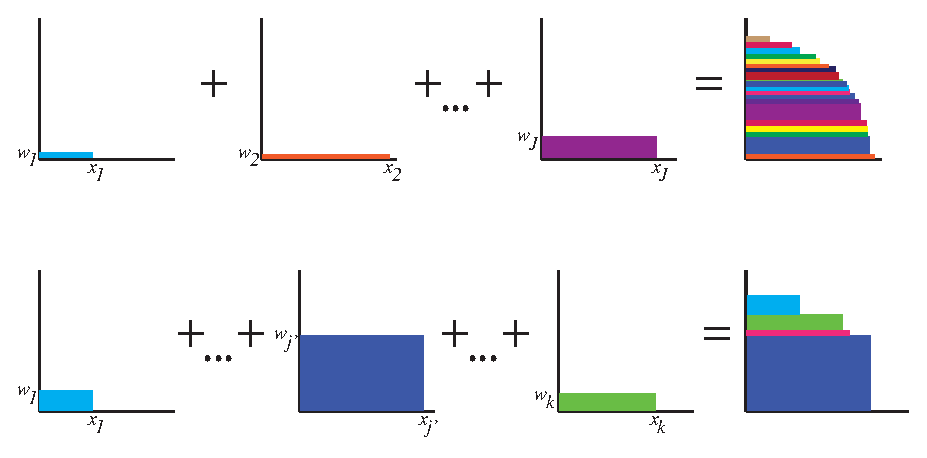
\includegraphics[width=\textwidth]{../FIGS/subset_blocks.eps} 
\caption{Conceptual depiction of loss exceedance curves from an event-based framework for a hypothetical example. For all subfigures, the X axis is \emph{$X$ = Performance measure} and the Y axis is the \emph{Annual rate of exceedance, $\lambda_{X>x}$}. The top row corresponds to an extensively-sampled event set including corresponding ground-motion intensity and damage maps. The bottom row corresponds to a subset of $k$ maps selected with the proposed optimization-based method, including re-weighting the occurrence rates, $w_{j'}$, of each map.}
\label{fig:blocks}
\end{figure*}

%more approach?
 To enable this optimization-based approach, we introduce two classes of network performance measures, proxy measures and target measures. The optimization procedure uses a proxy measure, since proxy measures ``serve as indirect measures of a given variable or process and are often used because of relative ease of measurement or understanding"~\cite{mckay_metric_2010}.  In contrast, target performance measures may be very computationally expensive. We choose a proxy performance measure to represent the target performance measure by combining ``soft'' knowledge, such as engineering experience, and an empirical method. Since the considered proxy network performance measure depends on the joint distribution of the ground-motion intensity, the proxy measure provides additional assurance that not only the target performance measure, but also the joint distribution of the ground-motion intensity, will be reasonably estimated. 
% 
%  help capture the joint distribution of the ground-motion intensity, because correlated losses usually correspond to high losses in network performance in contrast to independent component losses. Second, proxy measures can be chosen to be more strongly correlated to the target measure than the ground-motion intensity either by ``soft'' knowledge, such as engineering experience, or by an empirical method. %For example, if network failures result from component failures, this information can be used to choose a proxy measure related to component failures, which is a more direct relation to the network performance than the ground motion intensity. Alternatively, by using empirical correlation coefficients and limited tests, as will be discussed, we can empirically choose a proxy measure more correlated to the target performance measure than the ground motion intensity measure alone. 
 Finally, we describe a series of checks, a preliminary version of which we proposed in~\cite{miller_framework_2014}, to tune the model parameters to produce a final set of damage and ground-motion intensity maps. We also test that the final set is reasonably representative of an extensively-sampled baseline set of maps across various dimensions.
 
%%extensions (I'm thinking of discussing what the user would have and why I have correct answers)
To illustrate the proposed method, we assess the seismic risk to the San Francisco Bay Area road network with an event-based probabilistic loss estimation model. We show that by choosing maps based on spectral acceleration and a proxy performance measure (percentage of bridges damaged region-wide) in the objective function, we achieve low error for a more computationally intensive target performance measure (average percentage change in morning commute travel time). 
%gist of results

%significance
%This framework saves the researcher significant computational time in evaluating the seismic risk of infrastructure systems using event-based methods. Given the greater computational efficiency of our approach over other methods, the optimization framework enables better agreement between a risk estimate one would obtain from a full Monte Carlo analysis and some computationally tractable set of maps. 
Although the proposed framework requires formulating the optimization problem for the desired application and calculating proxy network performance measures for selecting a subset of damage and ground-motion intensity maps, the time invested in map selection is greatly outweighed by the expected savings in overall computational time for the risk analysis. The result is a more accurate and efficient probabilistic infrastructure network risk assessment.






\section{Risk framework}
\label{sec:framework}


\begin{figure}
\centering
\includegraphics[width=\textwidth]{../FIGS/subsets_maps.eps} 
\caption{Illustration of the risk framework for one earthquake scenario including: (a) One-second spectral acceleration  (ground-motion intensity) map with earthquake rupture, (b) bridge (component) damage map, (c) travel time increase (network performance measure) values. }
\label{fig:sample_pipeline}
\end{figure}

We perform an infrastructure network risk assessment in an event-based framework from earthquake scenarios to the final calculation of the network performance in three stages (e.g., Figure~\ref{fig:sample_pipeline}). First, we start with a set of earthquake scenarios based on a seismic source model, and then we generate ground-motion intensity maps (e.g., Figure~\ref{fig:sample_pipeline}{\color{red}(a)}).  Next, we sample realizations of  damage maps (e.g., Figure~\ref{fig:sample_pipeline}{\color{red}(b)}) and corresponding levels of functionality for the corresponding parts of the network.  Finally, we compute the network performance (e.g., Figure~\ref{fig:sample_pipeline}{\color{red}(c)}). At each stage, multiple realizations are possible, which will be discussed below. For illustration in Figure~\ref{fig:sample_pipeline}, we have shown one realization per stage.

%The analysis pipeline has 4 main steps: 1) We start with a set of ground motion scenarios based on a seismic source model. 2) We then generate ground-motion intensity maps and 3) draw realizations of damage maps. 4) Finally, we compute the network performance. 

This general risk analysis framework is common in academic literature and in practice~\cite{grossi_catastrophe_2005,johnson_planning_2005,jayaram_efficient_2010, han_probabilistic_2012,bommer_development_2002}. However, the last step, network performance, has varying treatment. For insurance applications, the loss calculated in the last step is simply the insured loss. This paper extends the prior work by detailing how to use optimization as part of a full risk framework to select a subset of maps for computing a target network performance measure and corresponding annual rates of occurrence.  These values enable a risk assessment of network performance losses.
% for a proxy measure. Through optimization, we are able to select a subset of ground motion maps and corresponding damage maps for which we do our final step, risk analysis using the target performance measure

% The diagram also shows how we will compare results of an optimized subset of intensity maps and an extensively-sampled baseline set of intensity maps. For purposes of illustration, we will consider seismic hazard and for the intensity measure will use the spectral acceleration at a period of $T=1s$, which is denoted by $\ln Sa(T=1s)$ or simply $\ln Sa$. 

\subsection{Ground-motion intensity maps}
We now describe how to produce a set of maps with ground-motion intensity realizations at each location of interest in a region and corresponding occurrence rates that reasonably capture the joint distribution of the ground-motion intensity. First, we generate $Q$ earthquake scenarios from a seismic source model. The seismic source model specifies the rates that earthquakes of specified magnitudes, locations, and faulting types will occur. This set of earthquake scenarios is comparable to a stochastic event catalogue in the insurance industry.

Second, for each earthquake scenario in the seismic source model, we use an empirical ground motion prediction equation (GMPE) to model the resulting intensity at each location of interest \cite[e.g.,][]{boore_ground-motion_2008,abrahamson_summary_2008,chiou_nga_2008,campbell_nga_2008}. The GMPE predicts the mean of the log ground-motion intensity, $\overline{\ln Y (M_q, R_{iq}, V_{s30,i}, \ldots) }$ and ground-motion intensity within- and between-event residual standard deviations, which are denoted by $\sigma_{iq}$ and $\tau_q$ respectively, for the $i^{th}$ site where $i = 1, \ldots, n$ in the $q^{th}$ earthquake scenario where $q=1, \ldots, Q$, $M_q$ is the moment magnitude of the $q^{th}$ scenario, $R_{iq}$ is the closest horizontal distance from the surface projection of the fault plane to location $i$, and $V_{s30,i}$ is the average shear wave velocity down to 30$m$ at the $i^{th}$ location. 

Then, for each of the $Q$ earthquake scenarios, we sample $b$ realizations of the spatially-correlated ground-motion intensity residual terms. Readers are referred to \cite{han_probabilistic_2012} for a survey of sampling methods.  Once residuals are sampled, the total log ground-motion intensity ($Y$) is computed as 

\begin{equation}
\ln Y_{ij} = \overline{\ln Y (M_j, R_{ij}, V_{s30,i}, \ldots) }+ \sigma_{ij} \epsilon_{ij} + \tau_j \eta_j
\label{eq:GMPE}
\end{equation}
where $j$ is the ground-motion intensity map index ($j = 1, \ldots, m$ where $m = Q \times b$), $\epsilon_{ij}$ is the normalized within-event residual in $\ln Y$ representing location-to-location variability and $\eta_j$ is the normalized between-event residual in $\ln Y$ and the other parameters are defined above. Both $\epsilon_{ij}$ and $\eta_j$ are normal random variables with zero mean and unit standard deviation. The vector of $\epsilon_{ij}$ can be modeled by a spatially-correlated multivariate normal distribution~\cite[e.g.,][]{jayaram_correlation_2009} %Boore et al. 2003; Wang and Takada 2005; Goda and Hong 2008; Jayaram and Baker 2009 
and the $\eta_j$ by a standard univariate normal distribution. 

The result is a set of $m$ ground-motion intensity maps (e.g., Figure~\ref{fig:sample_pipeline}{\color{red}(a)}). Since we simulate an equal number ($b$) of ground-motion intensity maps per earthquake scenario, the annual rate of occurrence for the $j^{th}$ ground-motion intensity map is the original rate of occurrence of the earthquake scenario, divided by $b$. We denote the final result as $w_j$.  

%The total log ground-motion intensity ($Y$) at the $i^{th}$ site for the $j^{th}$ ground-motion intensity map is the linear combination of the mean log ground-motion intensity and the residual terms, precisely
%\begin{equation}
%\ln Y_{ij} = \overline{\ln Y (M_j, R_{ij}, V_{s30,i}, T, \ldots) }+ \sigma_{ij} \epsilon_{ij} + \tau_j \eta_j
%\label{eq:GMPE}
%\end{equation}
%where $\epsilon_{ij}$ is the within-event residual in $\ln Y$ representing location-to-location variability and $\eta_j$ is the between-event residual in $\ln Y$ and the other parameters are defined above. The $\epsilon_{ij}$ can be modeled by a spatially-correlated multivariate normal distribution~\cite{jayaram_correlation_2009} %Boore et al. 2003; Wang and Takada 2005; Goda and Hong 2008; Jayaram and Baker 2009 
%and the $\eta_j$ by a standard normal distribution. 
%
%Our framework uses empirical ground motion prediction equations to generate realizations of ground-motion intensity. But, numerically simulated ground motions~\cite{graves_broadband_2010} could be used instead provided that the simulations provide intensity measure realizations at each site of interest and each simulation has an associated annual rate of occurrence.
%%Note that the resulting ground motion intensity maps show correlation from two sources, from correlation in the mean log spectral acceleration and correlation in the residual terms as discussed in \cite{baker_effects_2011}.

\subsection{Damage maps}
Calculating network performance risk requires assessing the structural response of relevant structures in the network to future earthquakes. The link between ground-motion intensity and structural response is often provided by fragility functions. Fragility functions express, for example, $P(DS_i \geq ds_s | Y_{ij} = y)$. We assume one component, such as a bridge, per site location, so we will identify both components and site locations via the index $i$. Using that notation, $DS_i$ is a discrete random variable whose value represents the damage state for the $i^{th}$ component and $ds_s$ is a damage state threshold of interest. The damage state is conditioned on a realization, $y$, of the random variable $Y_{ij}$, the ground-motion intensity at the $i^{th}$ site and $j^{th}$ ground-motion intensity map. Researchers have calibrated fragility functions using historical post-earthquake data~\cite[e.g.,][]{basoz_enhancement_1999}, experimental and analytical results~\cite[e.g.,][]{ramanathan_analytical_2010}, hybrid approaches, and expert opinion. Note that like the ground motion intensities, the damage states can be sampled from a joint distribution that includes correlation, such as due to similarities in design or construction practices~\cite[e.g.,][]{lee_uncertainty_2007,baker_introducing_2008}. 

By sampling a damage state for each component, with probabilities obtained from the fragility functions given the ground-motion intensity, we produce a damage map (e.g., Figure~\ref{fig:sample_pipeline}{\color{red}(b)}). The damage map has a realization of the damage state of each relevant component. This sampling process can be repeated multiple times to simulate multiple damage maps per ground-motion intensity map. For example, if equal numbers of damage maps are sampled per ground-motion intensity map ($c$ damage maps per ground-motion intensity map), the weight of the $j'^{th}$ damage map should be adjusted accordingly to $w_{j'}$, where $w_{j'} = \frac{w_j}{c}$, and $j' = 1, \ldots, J$. 

%These damage maps are directly mapped to the functionality of elements of the network. 
\emph{Functional percentage} relationships link the component damage to the functionality of network elements.  For example, in a road network, when a bridge collapses, the traffic flow capacity of the road it carries and it crosses can be modeled as reduced to zero. These relationships are often derived from a combination of observation and expert opinion, often due to data scarcity~\cite{werner_redars_2006}. Furthermore, the relationships are typically deterministic for a certain component damage state and restoration time~\cite{werner_redars_2006}. Thus, in this paper, each damage map corresponds to a functionality state for every element of the network.
%each damage map is directly mapped to the functionality of different elements of the network.
%each structure-component damage map corresponds to one network-component damage maps in this paper. Because the structure-component damage maps 
%
%we have defined the network-component damage maps structure-component damage maps co network-component damage maps , we will hereafter refer to structure-component damage maps as \

%For each intensity map, we generate \emph{component damage maps} with a discrete damage state at each location of interest sampled using appropriate fragility functions that provide a relationship between the $\ln Sa$ and damage states (Step 3 of Fig.~\ref{fig:pipeline}). 

\subsection{Network performance measures and risk analysis} \label{sec:net}
The final step for the event-based risk analysis is to evaluate the network performance measure, $X$. We will consider various network performance measures, each of which is a scalar quantity per damage map.  
%something about transportation
For road networks, two common performance measures are connectivity~\cite{basoz_bridge_1995,rokneddin_bridge_2013} and flow capacity~\cite{lee_post-hazard_2011}.  In order of increasing general computational cost, other measures to capture road network performance include the percentage of bridges damaged, weighted-shortest path between locations of interest \cite{chang_measuring_2001}, fixed-demand travel-time~\cite{stergiou_treatment_2006,shiraki_system_2007,jayaram_efficient_2010,han_probabilistic_2012}, morning or evening peak commute time, economic impacts from increased travel time and bridge repairs \cite{stergiou_treatment_2006}, and mode-destination accessibility~\cite{handy_measuring_1997}.  Fixed-demand travel time delay and its variants have become particularly popular in current literature (e.g., Figure~\ref{fig:sample_pipeline}{\color{red}(c)}).
%something about power
For power networks, connectivity is also a common network performance measure~\cite{duenas-osorio_seismic_2007}. Recently, power network researchers have introduced other measures such as serviceability ratio~\cite{adachi_serviceability_2008}, power system flow \cite{winkler_performance_2010}, and recovery time of the electrical network~\cite{shinozuka_seismic_2007}.
%something about water
Researchers have also used connectivity to measure the reliability of water networks with alternative measures including flow capacity, entropy-based measures, nodal demands, and the total number of component failures system-wide~\cite{romero_seismic_2010,hernandez-fajardo_sequential_2011,goulter_analytical_1995}.

Once the chosen performance measure is computed for each damage map, understanding the exceedance rate of different levels of performance is a common goal. The annual rate, $\lambda$, of exceeding some threshold of network performance is estimated by summing the occurrence rates of all damage maps in which the performance measure exceeds the threshold: 
\begin{equation}
\lambda_{X \geq x} = \sum_{j'=1}^{J} w_{j'} \mathbbm{I}(x_{j'}\geq x)
\label{eq:exceedance}
\end{equation}
where $x$ is a network performance measure threshold of interest and $x_{j'}$ is the network performance realization for the $j'^{th}$ damage map. The variable $w_{j'}$ is the occurrence rate of the $j'^{th}$ damage map as introduced above.
% ($w_j = \frac{w_j}{c}$ where $c$ is the number of damage map realizations per ground-motion intensity map). 
The indicator function $\mathbbm{I}$  evaluates to 1 if the argument, $x_{j'} \geq x$, is true, and 0 otherwise. By evaluating $\lambda$ at different threshold values, we derive an exceedance curve (e.g., Figure~\ref{fig:yirs}{\color{red}(b)}). In the results below, we will evaluate exceedance curves not only for the performance measure ($X$), but also for the ground-motion intensity measure ($Y$) (e.g., Figure~\ref{fig:yirs}{\color{red}(a)}). 



\section{Selecting a subset of maps}
\label{sec:selection}
\subsection{Damage and ground-motion intensity map selection problem}

\begin{figure}
\centering
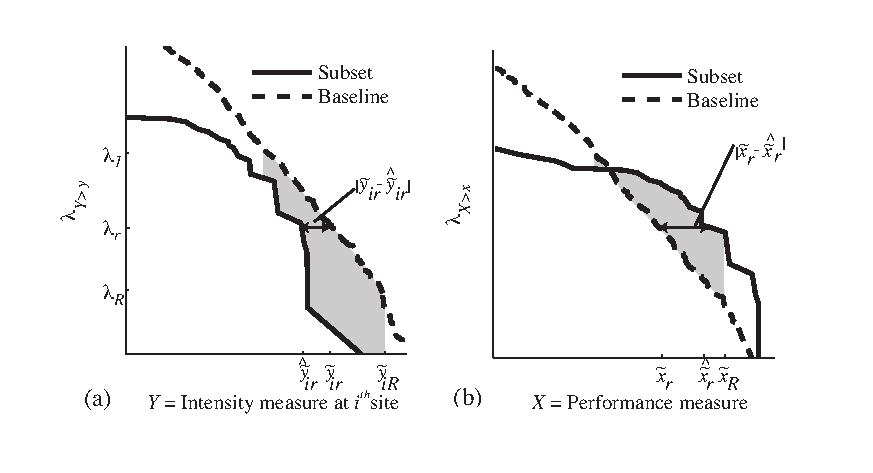
\includegraphics[width=5.6in]{../FIGS/subsets_yr4.eps} %VORSICHT: this is a hack. It should be 5.6 inches wide but somehow by importing it and saving it from Illustrator it shrunk so I had to reduce the width to keep the font size looking reasonable.
%\subfigure[Performance measure]{\includegraphics[width=2.8in]{../FIGS/yr.jpg}\label{fig:yr}} 
\caption{Relationship of error between the subset and the extensively-sampled baseline set of maps for (a) the empirical ground-motion intensity exceedance curves, and (b) the empirical performance measure exceedance curves. The solid line represents an example subset of maps chosen by optimization and the dotted line represents an extensively-sampled baseline set of maps. The grey-colored regions are related to the error and show where the curves differ; the optimization objective function minimizes the sum of the vertical distances between the curves.}
\label{fig:yirs}
\end{figure}

We now aim to choose a set of $k$ damage maps and corresponding ground-motion intensity maps, each with a corresponding adjusted annual rate of occurrence $w_{j'}$, from a set of $J$ candidate maps that provides a good representation of the earthquake hazard and performance risk. In other words, we want to approximate the profile of the loss exceedance curves of the ground-motion shaking intensity and performance measures. We do this by choosing a subset of damage maps and corresponding ground-motion intensity maps that minimizes the differences between the loss exceedance curves of an extensively-sampled baseline set and resulting subset over a range of return periods of interest. This region corresponds to error (shaded in  Figure~\ref{fig:yirs}). This can be expressed as:
%

%
\begin{subequations}
\label{eq:optim}
\begin{align}
\text{minimize} \notag \\
        & \alpha \| \diag{\boldsymbol\lambda}^{-1} (\boldsymbol\lambda - \Psi \textbf{w}) \|_1  + (1-  \alpha) \sum_{i=1}^{\nu} \| \diag{\boldsymbol\lambda}^{-1} (\boldsymbol\lambda - \Theta_i \textbf{w}) \|_1 \label{eq:objfunc} \\
    \text{subject to} \notag \\
        & \textbf{Card}(\textbf{w}) \leq k, \label{eq:const1}\\
        & \textbf{0} \leq \textbf{w}, \label{eq:const2} 
\end{align}
\end{subequations}
with variable $\textbf{w} \in \mathbb{R}^{J \times 1}$. Here each element of $\textbf{w}$, $w_{j'}$, represents the adjusted annual occurrence rate for the $j'^{th}$ damage map and corresponding ground-motion intensity map. The $\textbf{Card}(\textbf{w})$ denotes the cardinality (number of non-zero elements) of the vector $\textbf{w}$. The $\| \|_1$ represent the $L^1$-norm, which is simply the sum of absolute values of the vector. The vector $\textbf{0} \in \mathbb{R}^{J \times 1}$ is the vector of zeros. The vector $\boldsymbol\lambda$ is a vector of constants, $\lambda_1, \ldots, \lambda_R$; the elements of this vector represent the annualized exceedance rates, corresponding to $R$ discretized return period values, where the vector element corresponding to the $r^{th}$ return period equals $\frac{1}{\lambda_r}$.  The matrix $\diag{\boldsymbol\lambda}^{-1}$ is a matrix with all zeros except on the diagonals. 
Also, $\Psi  \in \mathbb{R}^{R \times J} $ is a matrix of constants, 
where for each entry of the matrix, $\psi_{r, j'} = \mathbbm{I}\{ x_{j'} \geq \tilde{x}_r \}$. The constant $\tilde{x}_r$ is the performance measure at the $r^{th}$ return period from an extensively-sampled set of damage maps ($\lambda_r = \lambda_{X \geq \tilde{x}_r}$).
% for return period indices $r  = 1, \ldots, R$. The constant $x_{j'}$ is the performance 
Similarly, $\Theta_i \in \mathbb{R}^{R \times J}$ is a matrix of constants corresponding to the $i^{th}$ site used in the objective function, where for each entry of the matrix, $\theta_{i, r, j'} =  \mathbbm{I}\{ y_{ij'} \geq \tilde{y}_{ir} \}$ for  $i$ denoting the indices of sites at which the objective function will be minimized ($i = 1, \dots, \nu$, where $\nu$ is less than or equal to $n$, the total number of sites of interest). The constant $\tilde{y}_{ir}$ is the ground-motion intensity value at the $r^{th}$ return period from an extensively-sampled set of ground-motion intensity maps (i.e., $\lambda_r = \lambda_{Y \geq \tilde{y}_{ir}}$).
Furthermore, the factor $\alpha$ in the objective function controls the contribution from the ground-motion intensity versus the performance measure. 

The objective function \eqref{eq:objfunc} minimizes the gaps between the exceedance rate curves from the baseline set and from the subset; each site considered in the objective function contributes a ground-motion intensity exceedance rate curve and the whole system also contributes one performance measure exceedance rate curve. Multiplying these values by $\diag{\boldsymbol\lambda}^{-1}$ in the objective function forces lower errors at larger return periods, typically of greatest engineering interest. The second term of the objective function  \eqref{eq:objfunc}, which sums up values related to the ground-motion intensity over all sites, corresponds to the objective function and definition of the error, as expressed as a constraint, in~\cite{han_probabilistic_2012}.
However, our new formulation includes an additional term related to the relatively computationally-cheap proxy performance measure (first term of  \eqref{eq:objfunc}). It also introduces the contribution factor $\alpha$. 
%Han and Davidson's mixed-integer optimization problem for selecting ground-motion intensity maps \cite{han_probabilistic_2012}; we introduce additional constraints to minimize the error in estimating the exceedance curve of a relatively computationally-cheap proxy performance measure,  describe the corresponding new variables, and simplify the expression for clarity. 
%Furthermore, we have reduced the number of variables by including the difference between the curves directly in the objective function; this reduction of variables can reduce computational effort. 
It also differs from most recent work in \cite{gearhart_optimization-based_2014}, because although the objective function in that work also contains a contribution factor and two terms, it considers marginal distributions of bridge damage state and the covariance in the bridge damage between pairs of bridges.  That work is limited to a single ground-motion intensity scenario; that optimization formulation does not explicitly consider consistency with the input distributions of the ground-motion intensity or network performance. This work, in contrast, considers uncertainty in the ground motion maps and uses a proxy network-wide performance in the objective function. We have also introduced a condensed form of the objective function and constraints, as compared to the more verbose mixed-boolean form in these other papers.

The first constraint  \eqref{eq:const1} specifies that the number of maps in the subset equals $k$. The second constraint \eqref{eq:const2} limits the value of each $w_{j'}$ to be non-negative, which is consistent with the physical interpretation of annual occurrence rates. 

%Because one of the constraints specifies that some of the variables must be binary integers, this is an example of a mixed-integer programming problem. 
Since the objective function and the second constraint are linear functions of the variables and constants---but there is a constraint on the cardinality of the set---this is an example of a convex problem with a cardinality constraint, which is nonconvex and NP-hard~\cite{boyd_l1-norm_2014}. %http://www.stanford.edu/class/ee364b/lectures/l1_slides.pdf
One general approach for solving this type of problem is branch-and-bound methods, which find a global solution to nonconvex problems by calculating upper and lower bounds on the optimal value for smaller and smaller parts of the domain of the random variables~\cite{lawler_branch-and-bound_1966,balakrishnan_branch_1991}. They maintain a provable upper and lower bound on the optimal value. While in the worst case the computational time grows exponentially with the number of random variables, in practice, the problem can require less computational effort~\cite{boyd_convex_2004}. The problem can also be solved through heuristics, as we will now discuss.

\subsection{Alternative ground-motion intensity map selection: relaxed problem with convex constraints}
\label{sec:alternativeSelect}
%The original problem~\eqref{eq:optim} has nonconvex constraints, $\textbf{Card}(\textbf{w}) \leq k$. 
To solve this problem more efficiently, we consider a convex relaxation of the map selection problem by replacing the nonconvex cardinality constraint~\eqref{eq:const1} with the convex constraints that  the sum of the $w_{j'}$ is less than or equal to $w_{tot}$, where the constant $w_{tot}$ is the sum of the original annual occurrence rates of all $J$ input maps. In other words, 
\begin{subequations}
\label{eq:optimb}
\begin{align}
\text{minimize} \notag \\
        & \alpha \| \diag{\boldsymbol\lambda}^{-1} (\boldsymbol\lambda - \Psi \textbf{w}) \|_1  + (1-  \alpha) \sum_{i=1}^{\nu} \| \diag{\boldsymbol\lambda}^{-1} (\boldsymbol\lambda - \Theta_i \textbf{w}) \|_1 \label{eq:objfuncb} \\
    \text{subject to} \notag \\
        & \| \textbf{w} \|_1 \leq w_{tot}, \label{eq:const1b}\\
        & 0 \leq \textbf{w}, \label{eq:const2b} 
\end{align}
\end{subequations}
where the parameters and variables are defined above.

This problem is now a convex optimization, because the objective function and the new constraint on $\textbf{w}$ are linear; it is an example of linear programming. One possible method for solving this  basic linear programming problem is an interior point solver~\cite{udell_bounding_2014,boyd_convex_2004}. An optimal value is guaranteed to exist~\cite{boyd_convex_2004}. Furthermore, the value of the objective function using these relaxed constraints provides a lower bound on the optimal value of the original formulation~\eqref{eq:objfunc}~\cite{boyd_convex_2004}. For testing the quality of the results, an upper bound on the original formulation~\eqref{eq:objfunc} could be found by a feasible solution; readers are referred to~\cite{udell_maximizing_2013,boyd_convex_2004} for more details.%section 3.1.5 of  S. Boyd and L. Vandenberghe, Convex Optimization. Cambridge,
%U.K.: Cambridge Univ. Press, 2004.

However, the solution to this problem is different from the original formulation~\eqref{eq:objfunc}, because there could be more than $k$ non-zero values. We adopt the heuristic method from Joshi and Boyd \cite{joshi_sensor_2009} to use the solution of the relaxed problem to select a subset. The maps with the $k$ largest weights are selected and then renormalized so that the sum of the $k$ new occurrence rates equals the cumulative annual rate of the input set of maps, $ w_{tot}$.  Upon implementation, the results are reasonably consistent with the baseline set and the errors using the original formulation. However, when the cardinality of the subset is very small, the chosen set of maps and corresponding annual occurrence rates tend to correspond to high error. We illustrate both trends in Section~\ref{sec:case}. Readers may also consider replacing $w_{tot}$ with a generic parameter and adjusting its value to force the number of non-zero $w_{j'}$ values to be less than $k$; the map selection problem here has parallels to the sparse signal reconstruction problem in Electrical Engineering~\cite{boyd_l1-norm_2014}. %slides 18-19 and 26-28 of http://www.stanford.edu/class/ee364b/lectures/l1_slides.pdf



%Since an
%SOCP problem is a convex optimization problem, a global solution of a mixed-integer second-order
%cone programming problem can be found by using, e.g., a branch-and-bound method; see, e.g.,
%Atamt�urk and Narayanan [4], Drewes and Pokutt [6] and Vielma et al. [32] for more account. This
%guaranteed global optimality is a major advantage of the proposed approach to the existing local
%and/or heuristic algorithms for design of damper distribution.
%
%make it more computationally feasible than the original formulation (eq.~\ref{eq:original}). However, it has the problem that it tends to produce results with a higher error at a very low desired number of maps, $k$, in the authors' experience. This will be illustrated in the case study below.

\subsection{Evaluation of error in the selected subset} \label{sec:errors}
We now evaluate the error in the estimation of exceedance rates between the selected subset of ground-motion intensity maps and the baseline set. A simple approach is to compute the value of the relevant term of the objective function of the optimization formulation. Alternatively, Han and Davidson \cite{han_probabilistic_2012} defined a Mean Hazard Curve Error (MHCE) for the ground-motion intensity as follows:
\begin{equation}
MHCE = \frac{1}{n R} \sum_{r=1}^R \sum_{i=1}^n \left| \frac{\tilde{y}_{ir} - \hat{\tilde{y}}_{ir}}{\tilde{y}_{ir}} \right|,
\label{eq:MHCE}
\end{equation}
where $\hat{\tilde{y}}_{ir}$ is the estimated ground-motion intensity using the selected subset of maps for the $r^{th}$ return period and $i^{th}$ site and the other variables have been defined above. This equation sums the normalized differences in the ground-motion intensity estimated from the subset and the baseline set over sites and return periods (Figure~\ref{fig:yirs}{\color{red}(a)}). 

We extend this error metric to evaluate the error in performance measure exceedance curves between the subset and the baseline set. This Mean Performance Measure Curve Error (MPMCE) is defined as 
\begin{equation}
MPMCE = \frac{1}{R} \sum_{r=1}^R \left| \frac{\tilde{x}_{r} - \hat{\tilde{x}}_{r}   }{\tilde{x}_{r}} \right|,
\label{eq:MPMCE}
\end{equation}
where $\hat{\tilde{x}}_{r}$ is the estimated performance measure value using the selected subset of maps for the $r^{th}$ return period and the other variables have been defined above (Figure~\ref{fig:yirs}{\color{red}(b)}). 



\section{Case study}
\vspace{-2pt}
\label{sec:case}
We illustrate the subset selection method with a case study assessing the seismic risk to the San Francisco Bay Area highway and local road network, as measured by the change in morning commute travel time for the 9-county region's approximately 7 million people~\cite{carr_study_2007}. 

\subsection{Dataset and models}

\subsubsection{Ground-motion intensity map models}

To generate a stochastic catalog of ground-motion intensity maps, we use the OpenSHA Event Set Calculator~\cite{field_opensha:_2003}. This software outputs the mean, $\overline{\ln Y_{ij}}$, and standard deviation values, $\sigma_{ij}$ and $\tau_j$, for all locations of interest for a specified seismic source model and ground motion prediction equation. The intensity measure is the 5\%-damped pseudo absolute  spectral acceleration ($Sa$) at a period $T=1s$, which is the required input to the fragility functions below. While our results use spectral acceleration, other intensity measures could be used to characterize the ground motion as long as a corresponding ground motion prediction model and spatial correlation model are available~\cite[e.g.,][]{foulser-piggott_predictive_2012}. %e.g., Foulser-Piggott and Stafford 2011). 
We use the UCERF2 seismic source model~\cite{field_uniform_2009}, Wald and Allen topographic slope model for the the shear wave velocity $V_{s30,i}$~\cite{wald_topographic_2007}, and the Boore and Atkinson \cite{boore_ground-motion_2008} ground motion prediction equation.   Using this seismic source model, which is then discretized into a list of faults and a stratified list of magnitudes and rupture locations for each, we obtain a set of 2110 earthquake events on active faults, and with annual occurrence rates greater than or equal to $10^{-5}$.


We simulate the baseline set of maps by combining the mean terms from the Event Set Calculator and spatially-correlated residual terms of the ground-motion intensity  (using~\cite{jayaram_correlation_2009}) according to the basic ground motion model~\eqref{eq:GMPE}. The baseline set has 5 residual realizations per ground motion scenario, which results in 10,550 ground-motion intensity maps (e.g., Figure~\ref{fig:sample_pipeline}{\color{red}(a)}).  We also generate two smaller sample sets of candidate ground-motion intensity maps that will be inputs to the optimization problem: one set with one residual realization per ground motion scenario (2110 maps total) and another with two residual realizations per ground motion scenario (4220 maps total). These two sets represent computationally-feasible set sizes for the optimization problem, and also enable testing the sensitivity of the optimization results to the input set size.

\subsubsection{Damage maps}%Description of network and its components} %includes bridge fragility and people exposure
We use a portfolio of 1743 highway bridges in the San Francisco Bay Area, which includes all unique state-managed bridges in current operation on the road network (illustrated in Figure~\ref{fig:sample_pipeline}{\color{red}(b)}). The bridges were hand-matched to road segments in the case study network (major roads illustrated in Figure~\ref{fig:sample_pipeline}{\color{red}(c)}).  If a bridge collapses, the road segment it carries, as well as that which it crosses, are modeled as closed. We do not include other types of failures, such as road damage from liquefaction, that may damage the network.

%We do not include other types of network component failures such as liquefaction in this study.

To compute damage to the bridges, we use fragility functions of the following form:
\begin{equation}
%$P(DS \geq ds_s | Y = y_{ij'}, i)$
P(DS_i \geq ds_s |Y_{ij} = y) = \Phi \left( \frac{\ln y - \lambda_{s, i}}{\xi} \right),
\label{eq:dsfull}
\end{equation}
where $\Phi$ is the standard normal cumulative distribution function, $\lambda_{s,i}$ and $\xi$ are respectively the mean and standard deviation of the $\ln Y$ value necessary to cause the $s^{th}$ damage state to occur or be exceeded, and $y$ is a realization of the random variable $Y_{ij}$, the ground-motion intensity at the $i^{th}$ site and $j^{th}$ ground-motion intensity map. The other variables are defined above.


The California Department of Transportation (Caltrans) provided the fragility function values $\lambda_{s,i}$ and $\xi$ used in this study. The values are based on structural characteristics including number of spans and structure age as detailed in \cite{basoz_enhancement_1999}.
%
% using the method detailed in \cite{basoz_enhancement_1999} based on The structural capacities of individual bridges are modeled as uncorrelated.

Per ground-motion intensity map, we compute one damage map (e.g., Figure~\ref{fig:sample_pipeline}{\color{red}(b)}), which has a realization of the bridge damage state at each bridge location according to the fragility function~\eqref{eq:dsfull}. The provided fragility functions do not consider correlation of the bridge capacities, but other models could be used~\cite[e.g.,][]{baker_introducing_2008}.

Each bridge damage state maps directly to the traffic capacity on associated road segments. We represent the road network by a directed graph $G = (V, E)$, where $V$ is a finite set of vertices representing intersections and the set $E$, whose elements are edges representing road segments, is a binary relation on $V$. Some edges (road segments) are matched to bridges, as described above. This study considers the Metropolitan Transportation Commission (MTC) \emph{Travel Model One} (version 0.3) of the San Francisco Bay Area transportation network where $(|V|, |E|) = (11921, 32858)$ including centroidal road segments and $(|V|, |E|) = (9635, 24404)$ without. Centroidal links refer to links that do not correspond to particular physical roads, but instead capture more subtle traffic flows, such as  from outside the study area, or the traffic flow to and from some minor local roads. The model includes both highways and main local roads as well as the relevant trip demand data. The travel origin-demand matrix for the latest run version, 2010\_03\_YYY, is from the MTC and is divided based on population density into 34 super districts covering the 9-county San Francisco Bay Area.

We use a functional percentage relationship to compute the traffic capacity of relevant road segments. Based on discussions with Caltrans, we consider travel conditions one week after an earthquake, since it is a critical period for decision making. For example, one week after most events, bridges should have been inspected and surface damage should be repaired, but major reconstruction would not have yet begun. According to our functional percentage relationship, at this point in time, the bridges have one of two classes of functionality, zero traffic capacity and full traffic capacity~\cite{werner_redars_2006}. We can thus summarize the bridge damage using two damage states $ds_s$, $ds_{damaged}$ and $ds_{functional}$, which correspond to the common HAZUS \emph{extensive} or \emph{complete} damage states and the \emph{none}, \emph{slight}, or \emph{moderate} damage states respectively~\cite{werner_redars_2006}. Thus, the functional percentage relationship assigns zero traffic capacity on road segments that have at least one bridge in the $ds_{damaged}$ damage state, and full traffic capacity otherwise. 



\subsubsection{Target network performance measures}\label{sec:perf}
We select the average change in morning commute time under fixed travel demands, which is proportional to the commonly-used fixed-demand travel delay for the same time period, as our target network performance measure. The morning commute time period is defined as 6am to 10am on weekdays. 

We estimate the trip time with the iterative traffic assignment (ITA) method \cite{chen_network_1991}, which has been shown by \cite{wang_understanding_2012} to be consistent with results from the commonly-used User Equilibrium (UE) method and to better estimate driver behavior because intuitively it captures drivers' choices of routes based on what traffic situation they currently see. We implement ITA according to the recommendations of \cite{wang_understanding_2012}  where the original demand matrix is divided into four parts, with 40\%, 30\%, 20\%, and 10\% respectively of the total trips. To begin, the first part of the trips are assigned using Dijkstra's algorithm to find shortest paths where the non-negative edge weights are the free-flow travel time ($t_f$). The resulting link flows ($q_f$) are recorded for each link. Then, we update the travel time ($t_a$) on each link according to the commonly-used formula, 
\begin{equation}
t_a = t_f \left( 1 + 0.15 \left( \frac{q_f}{c_f}\right)^{4}\right),
\end{equation}
where $c_f$ is the flow capacity of the link and the other variables are defined above~\cite{bureau_of_public_roads_traffic_1964}. Thus, travel time is a quartic function with link flow. Then, using these new free-flow times ($t_a$) as the edge weights, we use Dijkstra's algorithm to assign the second part of the trips. We repeat this approach until we have assigned all four parts of the trips.

We implement ITA in Python by leveraging the Python network analysis module NetworkX~\cite{hagberg_exploring_2008} (with some base algorithms in C and FORTRAN). The final result is a target performance measure and corresponding map (e.g., Figure~\ref{fig:sample_pipeline}{\color{red}(c)}) per ground-motion intensity map.

\subsubsection{Proxy network performance measures}
We now describe the selection of an appropriate proxy performance measure that is computationally inexpensive yet correlated with the target performance measure. We could select the performance measure by computing empirical correlation between the target and each candidate proxy measure for a computationally tractable number of scenarios. Another complementary strategy is to use other knowledge about the problem dynamics, such as in this case that the travel time should be related to bridge damage since the only network damage we are considering is directly related to bridges in a damaged state.  

To select a proxy performance metric for the case study, we randomly choose 10 ground-motion intensity maps and corresponding damage maps. For each damage map, we compute the values of the following candidate proxy performance measures: percent of bridges damaged, percent reduction in traffic flow capacity, and weighted-shortest path between locations of interest. 
%To select a proxy performance metric for the case study, we choose a set of 10 ground-motion intensity maps and corresponding damage maps for each for a group of candidate proxy performance measures, namely percent of bridges damaged, percent reduction in traffic flow capacity, and weighted-shortest path between locations of interest. 
To illustrate sensitivity to the initial set of scenarios, we provide the empirical $95^{th}$ percentile (point-wise) confidence interval by generating 100 realizations of 10 maps, sorting the empirical correlation values, and displaying the $5^{th}$ and $95^{th}$ percentile values (as well as the median) (Figure~\ref{fig:rhos}).  We find that \emph{percent of bridges damaged} is the proxy performance measure that across different quantiles on the confidence interval is most correlated with the target measure, which is corroborated by our engineering judgement. 
While we have provided the confidence interval to show the relative robustness of the method, it would not be calculated in practice because it is computationally expensive (namely requiring 100 sets of 10 evaluations of the target performance metric). We find that choosing just 10 random ground-motion intensity values and testing empirical correlation values provides insight into which proxy performance metric will be representative of the target performance metric. However, given some variability, particularly below the $50^{th}$ percentile values, this quantitative test should be supplemented with engineering judgement as described above. 


\begin{figure}[t!]
\centering
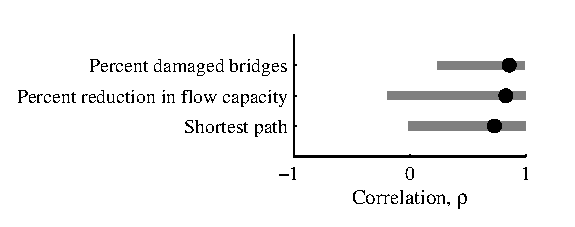
\includegraphics[width=3.75in]{../FIGS/subsets_rho.eps} 
\caption{Median (black dots) and empirical $95^{th}$ percentile point-wise confidence interval of the empirical correlation coefficient between candidate proxy performance measures and the target performance measure. Percent of bridges damaged is most highly correlated.}
\label{fig:rhos}
\end{figure}



\subsection{Map selection results and checks for consistency}
In this section, we select the optimization parameters, describe the resulting final subset of ground motion and damage maps, and then check the consistency of the results with the ground-motion intensity and performance measure rates of exceedance. 

\subsubsection{Final map selection} \label{sec:finalresults}
The optimization problem is solved using CVX, a Matlab package for specifying and solving convex problems \cite{grant_cvx:_2012, grant_graph_2008}, with the Gurobi Optimizer~\cite{gurobi_optimization_gurobi_2013}, for linear and mixed integer programming. We select maps using both the original nonconvex problem and the relaxed problem using convex constraints to compare their performance. The optimization problem~\eqref{eq:optim} is solved using a linear programming-based parallel branch and bound algorithm. The solver terminates (with an optimal result) when the gap between the lower and upper bounds of the objective function is less than 0.1\% of the upper bound~\cite{gurobi_optimization_gurobi_2013} or after 30 million iterations, whichever occurs first. Thus, in the numerical experiments here, the problem is solved using heuristics based on convex optimization. The relaxed problem using convex constraints~\ref{eq:optim} is also solved using CVX with the Gurobi Optimizer and terminates when an optimal solution is found. Supplementary information about the final map selection can be found in Appendix D of~\cite{miller_seismic_2014}. Furthermore, to facilitate adoption of the proposed methodology, Matlab implementations of both optimization-based map-selection methods are available at \href{http://purl.stanford.edu/wq017yv5965}{http://purl.stanford.edu/wq017yv5965}.

Next we set the relevant optimization parameters. In addition to the termination criteria, we have five main parameters to choose: the relative importance of ground-motion intensity versus the performance measure ($\alpha$), the number of return periods ($R$), the number of sites at which the objective function will be minimized ($\nu$), the number of candidate damage maps and corresponding ground-motion intensity maps ($J$ in general, which equals $m$ for the case study since $c=1$), and the desired number of ground-motion intensity maps in the final subset ($k$). 

We choose $k=25$ maps as a near-lower-bound case of the number of maps selected. In Section~\ref{sec:discussOpt} we will show results where $k=200$ maps for comparison with prior work.
% ($\frac{k}{2m + 2R(1+n)} < 0.02$ in the authors' experience)
With a small number of maps desired in the subset compared to the number of random variables, which is the case when $k=25$, we find that the alternative optimization formulation using convex constraints performs poorly. Since that method selects the scenarios with the $k$ highest renormalized annual rates, it excludes rare high intensity events, in practice, when the total number of maps ($k$) is very small. So, for the results below, we will use the original formulation~\eqref{eq:optim}. 

%However, when $k=200$ maps, we will show that near-identical subsets are selected using the original optimization problem and the alternative with convex constraints. Furthermore, the alternative finishes in a fraction of the time (hundredths of a second versus 70 seconds on a 2.8GHz desktop computer using the final parameters) and the result is guaranteed to be optimal.

We then determine the $\alpha, R, \nu$ and $J$ values empirically using grid search and computing the value of an evaluation function for each parameter combination (to ensure like comparisons, the evaluation function is $0.5$ MHCE $+ 0.5$ MPMCE(proxy) with 1743 sites and 50 return periods).  Grid search is a standard way of selecting parameters by exhaustively searching through a manually-specified subset of the parameter space. Note that while it may seem beneficial to use large values for $R, \nu$ and $J$, increasing the number of random variables makes convergence more challenging and can thus potentially increase error. Furthermore, there can be overfitting that causes MPMCE(target) to increase even as the objective function value decreases.


Via grid search, we determine our final set of parameters: $(\alpha, R, \nu, J, k) = (0.56, 50, 12, 2110, 25)$. The result of the original optimization problem~\eqref{eq:optim} using these parameters is the final output:  25 damage maps, corresponding ground-motion intensity maps, and associated annual occurrence rates. 

We will use this subset as an illustration; other subsets could have been selected with a different choice of parameter values or convergence criteria.  Furthermore, since computational time depends on the number of random variables, we find that in general, the choice of $J$ should capture, at least, the basic distribution of earthquake scenarios. The other parameter values can be explored using the grid search approach above, which we illustrated further in~\cite{miller_framework_2014}; one should include higher values in the parameter space (and thus a higher number of random variables), while the computation is feasible. Finally, note that the consistency checks below also help with tuning the parameters. This allows for leveraging any additional user expertise not  captured in the optimization formulation.


\subsubsection{Consistency checks}
We perform five checks: four  to evaluate how well the chosen set of ground-motion intensity maps and adjusted annual rates of occurrence represents the full joint distribution of $Sa$, and then one to test how well the selected subset and rates represent the baseline set of exceedance rates of the proxy performance measure.

%\renewcommand{\theenumi}{\Roman{enumi}}
\begin{enumerate}
\item \textbf{Fault sources} A possible pitfall is to primarily include events stemming from a major fault, such as the San Andreas Fault. In contrast, our subset still contains a range of faults, with no single fault contributing to more than 50\% of the annual rate of occurrence. Furthermore, since we constrain the ground-motion intensity maps inputted to the optimization to those with an annual occurrence rate of at least $10^{-5}$, we automatically have reasonably active faults in the final subset. 
\item \textbf{Magnitudes}  When we investigate the distribution of magnitudes, we see that the subset underestimates the rates at particularly low magnitudes. This behavior is not surprising because we have chosen to only match the exceedance curves between rates of 0.01 and 0.004 (return periods of 100 to 2500 years) and the low magnitude events are often more frequent, thus outside of the target range. However, there is a general good correspondence~\cite{miller_framework_2014}.

\item \textbf{Marginal distributions of ground-motion intensities} After looking at magnitudes, we compare the ground-motion intensity exceedance curves at individual sites. We compare results at two sites where the main contributors to the hazard are expected to be different  (Figure~\ref{fig:distributions}{\color{red}(c)}). The exceedance curves from the subset  fit reasonably well with the results from the baseline set, particularly between the return periods of 100 and 2500 years (e.g., Figure~\ref{fig:distributions}{\color{red}(a,d)}). This qualitative verification is corroborated by our overall error metric MHCE value~\eqref{eq:MHCE}, which averaged over all sites and 50 return periods is 30.3\%. For determining the size of a randomly-chosen set that, on average, gets the same error, readers can randomly select different size sets of ground-motion intensity maps and damage maps, normalize the $w_{j'}$, compute the error metrics, and compare~\cite{gearhart_optimization-based_2014}.
\item\textbf{Joint distributions of ground-motion intensities} 
The optimization has not explicitly considered the consistency of multivariate ground motion distributions when selecting the subset of maps.
However, we find that the realizations from the chosen subset and the baseline set are plausible pairings (Figure~\ref{fig:distributions}{\color{red}(b)}).
%It is not obvious that a stochastic catalog of ground-motion intensity maps that appear individually representative of different sites would still appear reasonable when considering a joint distribution. 
%However, we find that the empirical distribution from the subset relatively accurately defines the results from the extensively-sampled set, including skew (how balanced the distribution is on each side of the mean) and correlation (tightness of the simulation results band). 
This trend even appears for two sites where we might expect poor results because they have very different contributions to their ground motion hazard (Hayward Fault and San Andreas Fault, respectively, having major contributions). Thus, the results suggest that the optimization problem implicitly considers joint ground motion behavior because of the combination of minimizing error at each location individually and minimizing error to a region-wide metric that depends on joint bridge damage, and thus joint ground-motion intensities.
\item \textbf{Proxy performance measure} We see that the exceedance curve of the proxy performance measure~\eqref{eq:exceedance} using the selection results described in Section \ref{sec:finalresults} reasonably fits the exceedance curve of the baseline set (Figure~\ref{fig:pm}{\color{red}(a)}). This result corresponds to the summary error value of MPMCE(proxy) $= 7.1\%$ over 50 return periods and all 1743 locations. We do see that the subset underestimates the risk at return periods less than 100 years, which is outside the range of interest for the case study. If these return periods were of interest, then the return period parameters in the optimization could be adjusted accordingly.
\end{enumerate}
If the results are not as consistent for another application, one might try adjusting the parameters, for example, decreasing $\alpha$ to increase the contribution of fitting the marginal distributions of the ground-motion intensities in the objective function (or vice versa for the opposite effect), or increasing the total number of maps ($k$) used in the optimization. As the number of random variables is increased, one may also need to increase the relative gap and/or increase the maximum number of iterations associated with optimization termination. Thus, by following this step-by-step procedure and making any necessary adjustments, the modeler can be reasonably confident of the representativeness of the chosen subset for a seismic risk assessment of an infrastructure network.

\subsubsection{Target performance measure results}
Although the goal of the proposed selection procedure is to save computational time by not evaluating the target performance measure for the baseline set, for illustration, we will now compare results between the selected subset and the baseline set to test our set result. We find that the selected subset (ground-motion intensity maps, corresponding damage maps and occurrence rates) produces a reasonable estimate (Figure~\ref{fig:pm}{\color{red}(b)}). This corresponds to MPMCE(target) $= 2.7\%$ over 50 return periods. Also, as for the proxy measure, we observe that the estimate is most accurate within the return periods of interest included in the optimization. It may not be immediately obvious why MPMCE(target) is lower than MPMCE(proxy). This behavior stems from the definition of MPMCE that involves a sum of normalized differences in the performance metric between the exceedance curve from the baseline set compared to the exceedance curve from the selected subset (Section \ref{sec:errors}). The proxy metric has a larger range of values in the return periods of interest than the target metric so it comparably fares worse (Figure~\ref{fig:pm}). For example, if we instead include the target metric in the optimization formulation and test the subset on the proxy metric, we find that the error on the target metric decreases (since it is included in the optimization and it inherently has a lower range of values in the return periods of interest) while the error on the proxy metric increases (since it is not included in the optimization and there is a large range of values in the range of the return periods of interest). In conclusion, we see that the target performance measure results have relatively low error, even when the subset of damage maps is chosen only by the proxy performance measure and ground-motion intensity.
 

\begin{figure}[t!]
\centering
\includegraphics[width=5.6in]{../FIGS/subsets_distributions.eps} %subset_joints.pdf}
\caption[]{Ground-motion intensity exceedance curve comparison between the subset of ground-motion intensity maps where $k=25$ and the baseline set: (a) marginal exceedance curve at site B, (b) bivariate exceedance curve at sites A and B, (c) study map showing locations of sites A and B, and (d) marginal exceedance curve at site A. The grey box in panels (a) and (d) mark the range of the return periods of interest. }
\label{fig:distributions}
\end{figure}



\begin{figure}[t!]
\centering
\includegraphics[width=5.6in]{../FIGS/subsets_pm.eps} %subset_pm.pdf}
\caption{Comparison of the performance measure exceedance curves between the subset of ground-motion intensity maps where $k=25$ and the baseline set for (a) the proxy performance measure (percentage of bridges damaged), and (b) the target performance measure (percentage change in morning commute time). The grey box marks the range of return periods of interest.}
\label{fig:pm}
\end{figure}




\section{Discussion}
\vspace{-2pt}
\label{sec:discussOpt}
The case study demonstrates that an event-based approach to seismic risk analysis of a road network using optimization is feasible. In the following section, we discuss sensitivity to the choice of a target performance measure and the number of maps, as well as the role of numerically-calculated ground motions.
%\begin{figure}[t!]
%\centering
%\includegraphics[width=10cm]{../FIGS/k.jpg}
%\caption{Variation of error (MHCE, proxy MPMCE) with varying values of the number of maps in the final set of scenarios. TODO: replace.}
%\label{fig:k}
%\end{figure}

\subsection{Sensitivity to the choice of target performance measure}
We repeated the subset evaluation procedure with various other target performance measures to demonstrate that the performance of our method is not particularly sensitive to the choice of a target performance measure. Table \ref{table:others} shows the MPMCE(target) values for two alternative measures: (1) the estimated vehicle-miles traveled based on the previously-described demand data from the MTC and the ITA method and (2)  the weighted shortest path between locations of interest (here: points near the centroids of each of the 34 MTC superdistricts) according to the algorithm by \cite{chang_measuring_2001} where the edge weights for Dijkstra's shortest path algorithm are the free-flow travel times, which we also implement in Python using the NetworkX module. The results indicate that the results remain relatively robust with a change of target performance measure. 
% (1) We compute the traffic flow capacity between two points of interest (San Francisco and Oakland) using the max-flow algorithm where the edge weights are the damaged or undamaged traffic flow capacity for each road link as implemented in Python in the Networkx module. 
%As the table shows, the results were similar and in some cases better than the performance of the originally chosen target performance measure. 

%rows are the w.m. columns are method 1 and method 2
\begin{table}
\centering
\begin{tabular}{l*{1}{c}r}
\hline
\hline
Performance measure             & MPMCE $(\%)$ \\
\hline
\textbf{Morning commute travel time}           & 2.7  \\
Vehicle-miles traveled     & 1.8  \\
Shortest paths     & 5.1  \\
\hline
\hline
\end{tabular}
\caption{Mean performance measure curve error (MPMCE) for various target performance measures. All results use the same subset of maps in the case study optimization result where the parameters are $(\alpha, R, \nu, J, k) = (0.56, 50, 12, 2110, 25)$.}
\label{table:others}
\end{table}

\subsection{Extension to other target number of maps}
We have shown results for $k=25$ maps in the case study to test the limits of our approach. A more common choice of $k$ in recent literature is around 200 maps  \cite{han_probabilistic_2012, jayaram_efficient_2010}. As expected, we see a reduction in the error when $k=200$.
% (Figure~\ref{fig:k}). 
The MHCE drops from 30.3\% to 14.9\%, the MPMCE(proxy) from 7.1\% to 4.9\%, and the MPMCE(target) from 2.7\% to 0.9\%. Visually we see a closer match of the subset and baseline loss exceedance curves when $k=200$, which corroborates these quantitative error metrics. These results suggest that it is beneficial to increase $k$ as much as is computationally feasible for the final application of the chosen subset. However, reasonable results can still be achieved with a relatively small number of maps.

In addition, when $k=200$ maps,  the original optimization problem and the alternative with convex constraints select nearly identical subsets. Furthermore, the alternative finishes in a fraction of the time (hundredths of a second versus 300 seconds on a 2.8GHz desktop computer using the final parameters) and the result is guaranteed to be optimal with respect to the associated objective function and constraints.

\subsection{Role of numerically-calculated ground motions}
We have considered a simulated set of ground motions using empirical ground motion models. This framework could easily be adapted for a stochastic catalog of numerically simulated ground-motion intensities such as hybrid-broadband simulations~\cite[e.g.,][]{graves_broadband_2010}. By repeatedly simulating ground-motion intensities at each location over a large number of rupture scenarios, the above analysis could be repeated. While creating such a stochastic catalog is potentially computationally expensive, the results could serve as useful validation of a seismic risk assessment using the empirical ground motion models, or as an alternative to consider.




\section{Conclusions}
\vspace{-2pt}
\label{sec:conclusionsOpt}
We have presented a computationally efficient method for selecting a subset of damage maps, corresponding ground-motion intensity maps, and associated occurrence rates for a probabilistic infrastructure network risk assessment using optimization.
%significance/advance
%The approach introduces a constraint on the exceedance rate consistency of a performance measure when selecting a subset of ground-motion intensity maps. This implicitly captures the joint distribution of the spectral acceleration in the optimization objective function.
Through a case study of the San Francisco Bay Area road network, we have demonstrated how to use the optimization formulation to select a subset of damage maps (with corresponding ground-motion intensity maps and occurrence rates) from a larger set of candidate maps. The problem minimizes the error in estimating the marginal distributions of ground-motion intensity at individual locations as well as the distribution of a proxy network performance measure (percentage of bridges damaged).  The proxy performance measure implicitly captures the joint distribution of the spectral acceleration in the optimization objective function. Furthermore, we describe checks of consistency with the ground motion hazard such as fault distribution and discuss the error in estimating the exceedance curve of the proxy performance measure and of the target performance measure (percentage change in average morning commute time). We have shown that the results from the subset are a good estimate of the results from an extensively-sampled baseline set of maps. 
%more significance
Thus, the researcher or decision maker can estimate the exceedance rates of a target performance measure with a reduced subset of damage maps while still achieving reasonable accuracy. This is significant, because many performance measures are extremely computationally expensive to evaluate. Thus, this work can be used to transform a ``what-if'' scenario approach into one using an event-based probabilistic loss estimation model for assessing risk efficiently. With this improved understanding, researchers and policy makers can better mitigate risks and increase community  resiliency. 
Additionally, this work aids emergency response planning by identifying a small, but representative, set of scenarios to consider in planning exercises.
%Another significance of this work is emergency response planning. By identifying a small number of scenarios corresponding to a range of network performance outcomes, this method may improve emergency response planning by pointing out scenarios to simulate for emergency response preparedness. For example, in the final set of 25 maps in the case study, three scenarios at equal intervals of traffic network performance are the less disruptive M6.45 Calaveras fault event, moderately disruptive M7.15 Calaveras fault event, and extremely disruptive M8.05 N. San Andreas fault event. %6.95 Hayward Rogers-Creek
%applications
Finally, this approach can potentially be applied to efficiently analyze risk from other natural hazards impacting networks.


\acks
We thank Dave Ory at the Metropolitan Transportation Commission (MTC), and Tom Shantz and Loren Turner at Caltrans for motivating discussions and providing the case study network data. We also gratefully acknowledge Madeleine Udell of Stanford University for her help with the condensed optimization formulation and discussion in Section 3; the manuscript is greatly improved based on her feedback. We also thank Jessica Jacobo of the University of California-Berkeley for painstakingly integrating the Caltrans and MTC data. She reconciled the approximate geographic coordinates provided for bridges with the 3D locations of the road segments, using estimated geographic coordinates of the road segments, text descriptions, and aerial images. Furthermore, thanks to the anonymous reviewers for helpful feedback. MTC develops and maintains a regional travel model for regional planning purposes.  As a public agency, the MTC sees the model as a public good and welcomes its use by others.  However, the authors are entirely responsible for the use of the model in the present context, including assessing the reasonableness of the results for the task at hand.  MTC has not reviewed and does not endorse the model results, implicitly or otherwise. Also, the first author gratefully acknowledges the support of the Stanford Graduate Fellowship and the National Science Foundation Graduation Research Fellowship. This work was supported in part by the National Science Foundation under NSF grant number CMMI 0952402. Any opinions, findings and conclusions or recommendations expressed in this material are those of the authors and do not necessarily reflect the views of the National Science Foundation. 


\bibliographystyle{wileyj}	% (uses file "plain.bst")
\bibliography{newfile} %subset_journal} %change via grep -v "url =" subset_journal.bib > newfile.bib %http://tex.stackexchange.com/questions/26318/disabling-urls-in-bibliography

\end{document}
